%
%TODO change pictures from png to pdf
%
%
%\defcitealias{Mao0130669431ISBN}{Modern Cryptography: Theory and Practice.}
\chapter{Programovatelné hradlové pole - FPGA}
\section{FPGA}
Programovatelná hradlová pole, neboli FPGA byli prvně představeny v 80. letech společností Xilinx, Inc. Do nedávna byly FPGA používány k prototypovaní a~emulacím při procesu návrhu a výroby integrovaných obvodů určených pro aplikaci tzv. ASIC.\cite{Sekanina3540403779ISBN}
Nicméně v~poslední době se FPGA čipy rozšířily mimo návrh ASIC obvodů a~jsou vyráběny v~mnoha variantách pro různá odvětví. Hlavní výhodou obvodů FPGA je možnost následného přeprogramovaní i~po jejich výrobě.\cite{FPGAfromMIT}

FPGA se skládají z~tří hlavních typů programovatelných stavebních bloků. Rozložení těchto tří bloků je zobrazeno na \obrazek{img:Architektura}.
\begin{figure}[!h]
  \begin{center}
    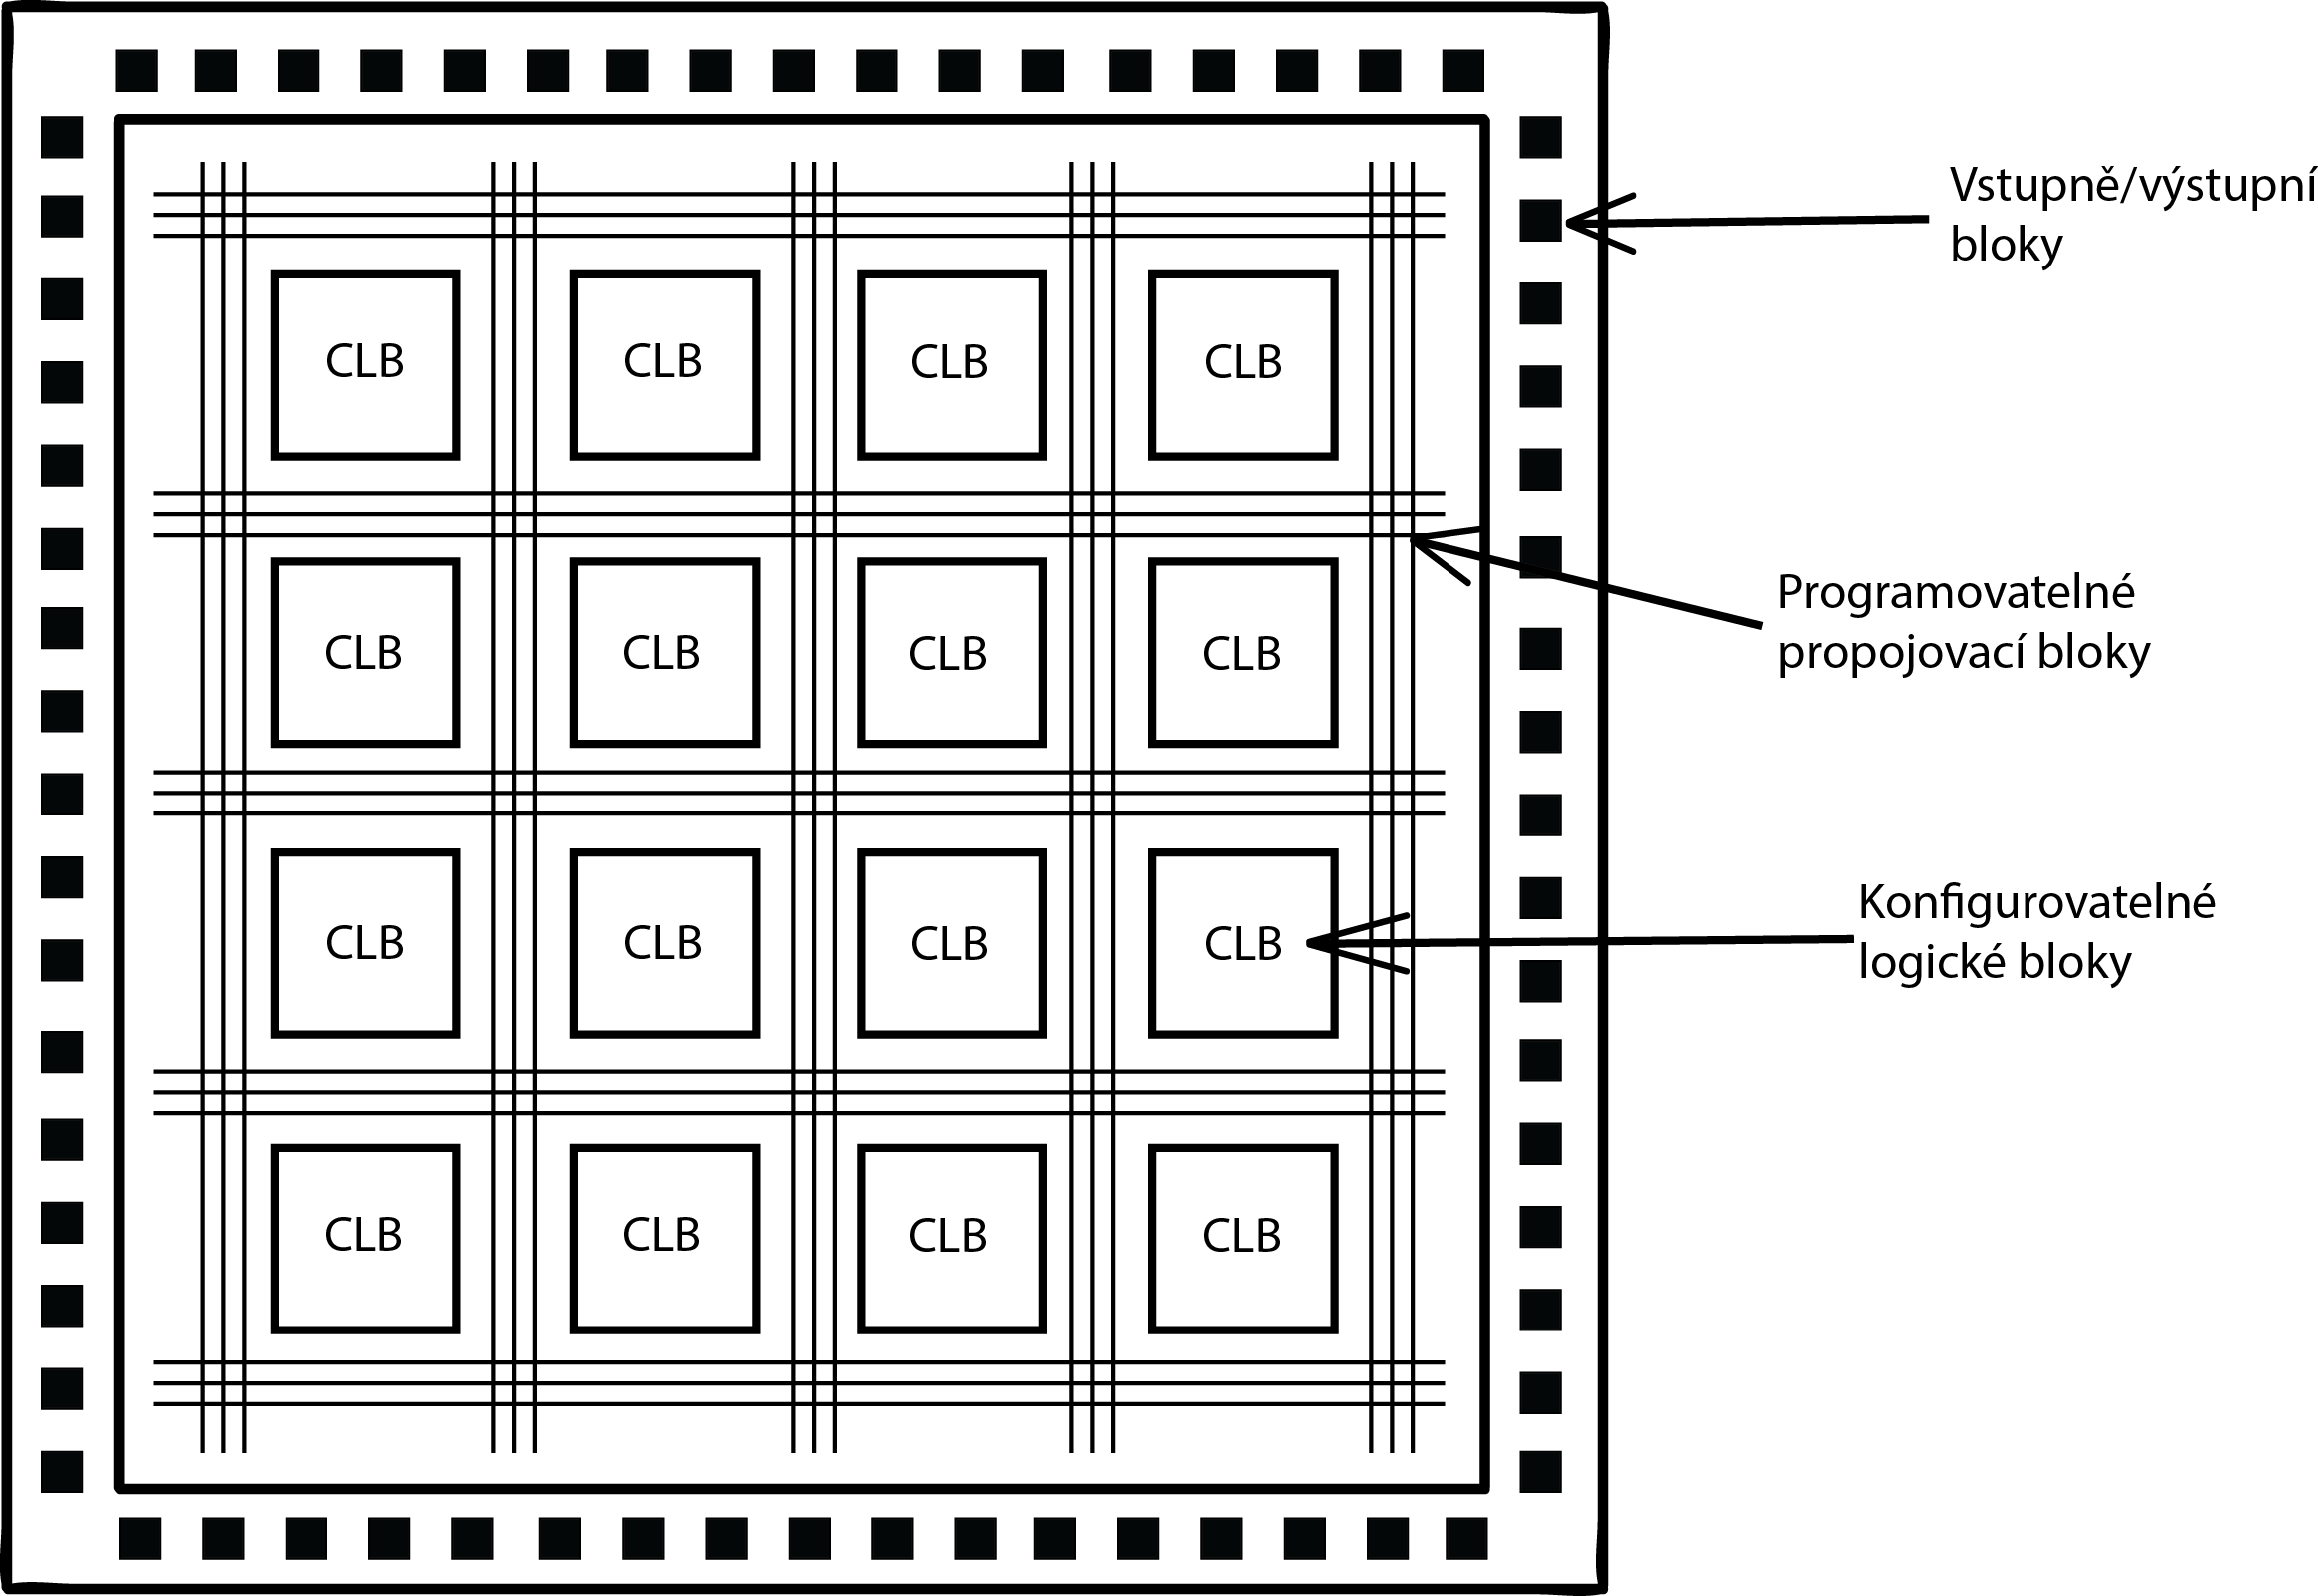
\includegraphics[scale=0.5]{obrazky/FPGA-architekrura-vlastni.png}
  \end{center}
  \caption[Architektura FPGA]{Architektura FPGA čipu \cite{electronicshub.org}}
  \label{img:Architektura}
\end{figure}
\begin{itemize}
    \item IOB - vstupně/výstupní bloky
    \item PIB - programovatelné propojovací bloky
    \item CLB - konfigurovatelné logické bloky
\end{itemize}

CLB mohou být naprogramovány tak, aby implementovaly různé logické funkce. Při propojení pomocí PIB vytvářejí velké logické okruhy. Vstupně výstupní bloky IOB propojují interní a externí zdroje. Na FPGA čipu se dále nachází SRAM\footnote{Statická paměť.\label{foot:sram}}, která uchovává konfiguraci CLB, PIB a IOB bloků.\cite{Sekanina3540403779ISBN}
%TODO bakalarka rozvest na vic teorie detailnejsi popsani co je LUT atd
\setcounter{footnote}{0}
\section{Xilinx Zynq-7000}
Čipy z~rodiny Zynq-7000 nabízí flexibilitu a~škálovatelnost FPGA čipů, zatímco poskytují sílu, výkon a použitelnost, která je často spojována s~ASIC čipy.
O~výpočetní sílů se stará processing system (PS), který je založen na technologii ARM$\copyright$\footnote{Advanced RISC machine je typ procesoru, který má zmenšenou sadu instrukcí a~není energeticky náročný.\label{foot:ARM}} Cortex\textsuperscript{TM}-A9, který obsahuje paměť přímo na čipu, rozhraní pro externí paměť a~sadu periferních rozhraní. FPGA se často označuje jako programmable logic (PL), kde pro Zynq-7000 je založen na bázi 28nm výrobního procesu od firmy Xilinx. Výhodou rodiny Zynq-7000 je, že processing system a~programmable logic jsou integrovány na jednom čipu. Touto integrací lze dosáhnout většího výkonu než když jsou tyto dvě části rozděleny na více čipech. Vývoj pro všechny typy programmable logic od Xilinxu probíhá v~prostředí Vivado Design Suite.\cite{Zynq-7000}
\begin{figure}[!h]
  \begin{center}
    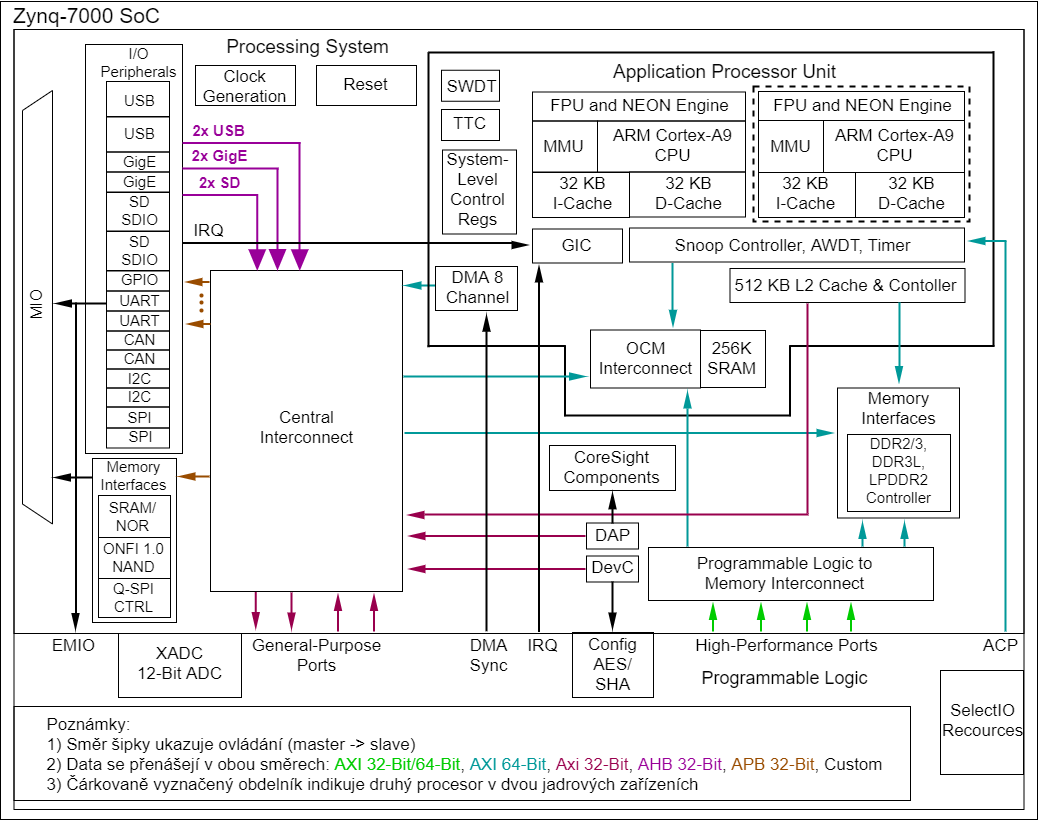
\includegraphics[scale=0.4]{obrazky/Zynq-7000-own.png}
  \end{center}
  \caption[Architektura Zynq-7000]{Architektura Zynq-7000 čipu \cite{Zynq-7000}}
  \label{img:Zynq-7000}
\end{figure}
% done 17.10.2020
\chapter{Kryptografie}
\section{Základní pojmy}
\textbf{Kryptologie} je věda zabývající se konstrukcí a překonáváním matematických metod zajištující důvěrnost a~autentičnost zpráv. Tato věda v sobě obsahuje kryptografii a~kryptoanalýzu.\newline
\textbf{Kryptografie} je věda zabývající se konstrukcí matematických metod pro zajištění důvěrnosti a~autentičnosti zpráv.\newline % burda aplikovaná
\textbf{Kryptoanalýza} je věda zabývající se překonáváním matematických metod, které zajišťují důvěrnost a~autentičnost zpráv.\newline % burda  aplikovaná
\textbf{Kryptografický systém} zkráceně kryptosystém je systém algoritmů, který zajištuje důvěrnost a~autentičnost zpráv.\cite{Burda9788021446120ISBN}\newline
\textbf{Klíč} je parametr procesu šifrovaní a~dešifrovaní.\cite{Burda9788072049257ISBN}\newline %burda
\textbf{Zpráva} jsou vstupní data, která jsou potřeba šifrovat, někdy označována jako čistý nebo prostý text.\cite{Mao0130669431ISBN}\newline % wenbo mao
\textbf{Šifrovaný text} jsou výstupní data z procesu šifrovaní, která jsou v~nečitelné podobě.\newline % burda
\textbf{Šifra} je určitý postup neboli algoritmus pomocí kterého se šifruje a~dešifruje zpráva.\cite{Burda9788072049257ISBN}\newline
\textbf{Šifrování} je proces transformace určité zprávy do nečitelné podoby.\cite{Mao0130669431ISBN}\newline % wenbo mao
\textbf{Šifrátor} je zařízení, které šifruje zprávu pomocí šifry na šifrovaný text.\newline
\textbf{Dešifrování} se nazývá opačný proces šifrovaní neboli přetváříme šifrovaný text na původní zprávu.\cite{Mao0130669431ISBN} %wenbo mao  
%\section{Historie} TODO bakalařka
\section{Princip kryptosystémů}
V~roce 1883 Auguste Kerchoffs sepsal podmínky pro vytváření kryptosystémů, kde jedna z~podmínek se rozšířila a~stala se uznávanou konvencí známou jako Kerchoffsův princip. Který říká: \newline\begin{quote}
    \textit{\uv{Znalost algoritmu a~velikosti klíče stejně jako dostupnost známého prostého textu jsou standardní předpoklad v~moderní kryptoanalýze. Protože útočník může tyto informace případně získat, není proto dobré se spoléhat na jeho utajení při posuzovaní jeho kryptografické síly.\footnote{Přeloženo z anglického jazyka, originální znění~v \citace{Modern Cryptography na straně 208}{\cite{Mao0130669431ISBN}}}}}
\end{quote}
\newpage
Propojením Kerchoffsova principu a~Shannonovy teorie informace lze poskytnout shrnutí pro dobrý kryptografický systém.
\begin{itemize}
    \item Algoritmus by neměl obsahovat žádnou část, která je tajná.
    \item Rozložení informace v zašifrovaném textu by mělo být po celé délce rovnoměrné až náhodné.
    \item Správný klíč by měl zaručit, aby šifrování a~dešifrování bylo efektivní.
    \item Velikost klíče by měla udávat náročnost na dešifrování zašifrovaného textu bez použití správného klíče.\cite{Mao0130669431ISBN}
\end{itemize}

\section{Hašovací funkce}
\label{sec:hashFunction}
Jednosměrné funkce jsou takové, pro které lze vypočítat obraz funkce, ale z~obrazu by nemělo být možné vypočítat vzor obrazu. Jednosměrné funkce se dělí na funkce s~volitelnou a~pevnou délkou výstupu.\cite{Burda9788021446120ISBN} % burda
Skupina s pevnou délkou výstupu se nazývá hašovací funkce. Hašovací funkce pracuje na principu, kde vstup je bitový řetězec proměnné délky a~výstupem je řetězec o~konstantní bitové délce takzvaný haš\footnote{Často označován anglicky hash}.\cite{Mao0130669431ISBN}%mao
\newline
Od hašovacích funkcí jsou zpravidla požadovány tyto vlastnosti:
\begin{itemize}
    \item Odolnost vůči získaní vzoru
    \item Odolnost vůči modifikaci vzoru
    \item Odolnost vůči kolizím
    \item Efektivita
\end{itemize}
\begin{figure}[!h]
  \begin{center}
    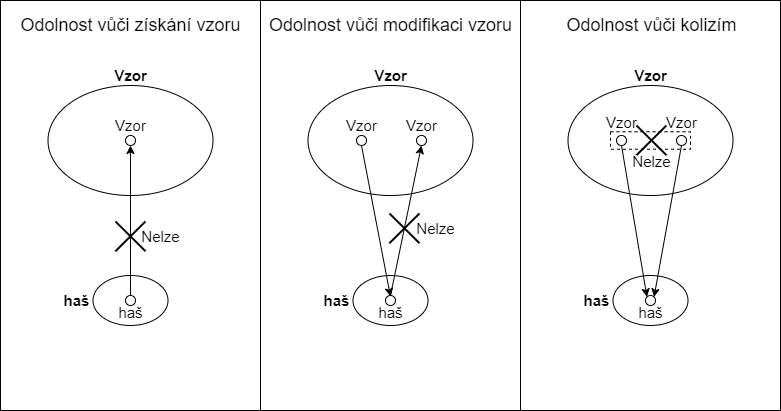
\includegraphics[scale=0.4]{obrazky/HashFunction.png}
  \end{center}
  \caption[Požadované vlastnosti haš funkce]{Požadované Vlastnosti haš funkce.\footnotemark\cite{Burda9788021446120ISBN}}
  \label{img:HashFunction}
\end{figure}
\footnotetext{Obrázek lze nalézt v \citace{Aplikovaná kryptografie na straně 53}{\cite{Burda9788021446120ISBN}}}
Jednosměrnost neboli odolnost vůči získaní vzoru by měla splňovat, že z~množiny hašů by nemělo být prakticky možné nalézt vzor, pro který by platila funkce H(vzor)\,=\,haš, kde H je hašovací funkce.

Odolností vůči modifikaci vzoru se požaduje, aby prakticky bylo téměř nemožné po %TODO kontrola
vypočtení haše z prvního vzoru nalézt druhý vzor, který by měl stejný haš.

Při odolnosti vůči kolizím by mělo být téměř nemožné najít dva rozdílné vzory pro které by vycházel stejný haš.\cite{Burda9788021446120ISBN} %burda

Pro splnění efektivnosti by daná hašovací funkce měla být realizovatelná v polynomiálním čase, nejlépe však v lineárním.\cite{Mao0130669431ISBN} %mao

Nejčastější využití hašovacích funkcí nalezneme v~digitálních podpisech, kryptografických aplikacích generujících pseudonáhodné data a~asymetrických kryptosystémech. V digitálních podpisech je hašovací funkce použita k~vytvoření otisku zprávy, který slouží k~ověření autentičnosti a~integritě. Generace pseudonáhodných dat se využívá ve spoustě případů od autentifikačních protokolů po protokoly elektronické komerce. V asymetrických kryptosystémech se používá k~ověření správnosti šifrovaného textu. Tento mechanizmus je nezbytný k~zabezpečení ochrany proti útokům.\cite{Mao0130669431ISBN}%mao
%done 20.10.2020
\section{Asymetrická kryptografie}
Asymetrická kryptografie někdy nazývaná kryptografie s~veřejným klíčem používá dva rozdílné klíče. Tyto klíče se nazývají veřejný klíč označovaný jako \uv{public key} a~soukromý klíč označovaný jako \uv{private key}. Veřejný klíč se používá k~šifrovaní zprávy a~soukromý klíč k dešifrovaní zašifrované zprávy pomocí veřejného klíče. Hlavní silou této metody je, že příjemce vypočítá veřejný a~soukromý klíč, ale sdílí pouze veřejný. Odesílatel pomocí asymetrické šifry a~veřejného klíče šifruje zprávu, kterou následně pošle příjemci, který vydal veřejný klíč. Příjemce pomocí soukromého klíče dešifruje přijatou zprávu. Výhoda této metody spočívá v~tom, že při odeslání špatnému příjemci nebo odcizení zprávy by neměl nesprávný příjemce dešifrovat zprávu bez znalosti soukromého klíče. Tyto dva klíče jsou propojené složitými matematickými výpočty, kdy veřejný klíč nenese informace o~soukromém klíči. Z tohoto důvodu při požadavcích kladených na bezpečnost v~dnešní době v~reálném čase není možné vypočítat z~veřejného klíče soukromý klíč. Nejznámější a~nejpoužívanější šifrou je RSA
(Rivest–Shamir–Adleman).\cite{Nigel9780077099879ISBN}
\newpage
% todo obrázek od mao page cca 209
\begin{figure}[!h]
  \begin{center}
    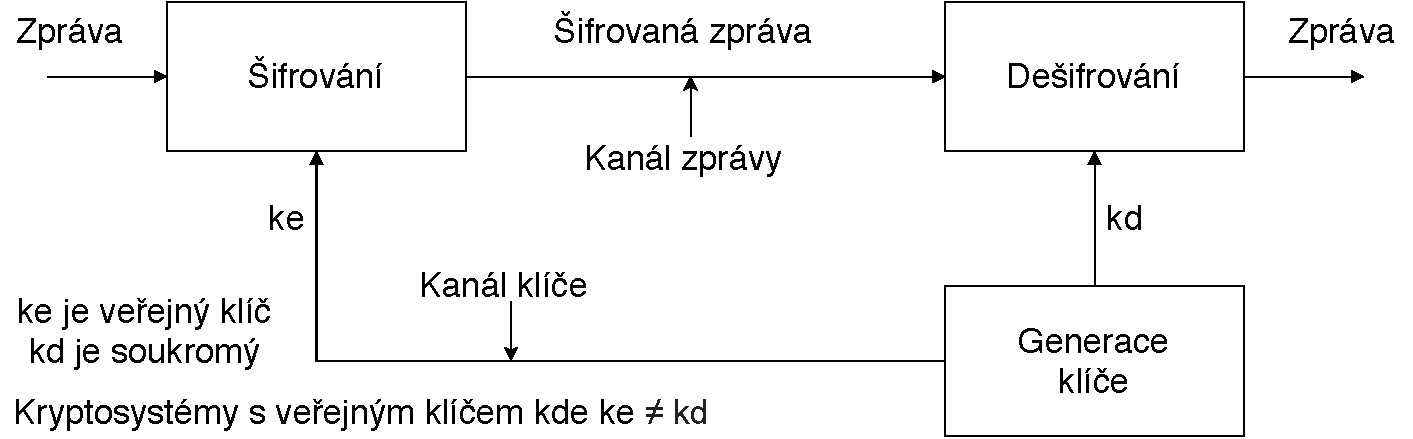
\includegraphics[scale=0.5]{obrazky/AsymmetricCrutosystem.pdf}
  \end{center}
  \caption[Princip asymetrického kryptosystému]{Princip asymetrického kryptosystému.\footnotemark\cite{Mao0130669431ISBN}}
  \label{img:asymmetricCrypto}
\end{figure}
\footnotetext{Obrázek lze nalézt v \citace{Modern Cryptography na straně 208}{\cite{Mao0130669431ISBN}}}
% todo bakalářka doplnit teorii
\section{Symetrická kryptografie}
Symetrická kryptografie se odlišuje od asymetrické kryptografie počtem klíčů, kdy symetrická kryptografie využívá pouze jednoho soukromého klíče, který slouží pro šifrovaní a~dešifrovaní. Tento klíč si obě dvě strany, které chtějí komunikovat, musejí vyměnit. Problém může nastat při ustanovení a~výměně klíče, kde lze klíč jednoduše odchytit pokud spojení není zabezpečené. Bezpečná výměna a~ustanovení klíče může proběhnout fyzickou výměnou, která v~moderní době není možná v~globálním měřítku. Při ustanovení a~výměně klíče se přes nezabezpečenou síť využívá asymetrické kryptografie. V~některých případech symetrické algoritmy využívají dva klíče -  jeden k~šifrovaní a~druhý k~dešifrovaní. Při odcizení šifrovacího klíče lze jednoduše vypočítat dešifrovací klíč a naopak. Jelikož se při vytváření šifry počítá, že algoritmus na ustanovení klíčů je veřejně známý, měl by být rozsah klíčů velmi velký. Pokud je rozsah klíčů malý, lze jej prolomit hrubou silou. Symetrické šifry dělíme na proudové a~blokové.\cite{Nigel9780077099879ISBN}

\subsection{Proudové šifry\label{subsec:streamFunction}}% možná podsekce symetrických
Mezi hlavní výhody proudových šifer patří bezchybovost nebo velice malá chybovost. Tyto šifry musí zpracovávat proud bitů a každý bit se šifruje samostatně. Oproti blokovým šifrám jsou rychlejší a~méně hardwarově náročné. Lze je rozdělit na dva typy. Prvním typem jsou synchronní a~druhým jsou asynchronní. Rozlišujeme je podle generace takzvaného keystreamu, což je generující klíčový proud znaků.\cite{HavlicekBakalarka}

U~synchronních proudových šifer nezáleží na šifrovaném a~nešifrovaném textu při generaci keystreamu. Generace keystreamu je pouze závislá na klíči a~šifrovacím algoritmu, ke kterému se u~moderních šifer přidává ještě inicializační vektor (IV).\cite{EncyclopediaSynchronous} Jedním z~požadavků na takovou šifru je synchronizace odesílatele a~příjemce, to znamená, že každá strana musí mít stejný stav algoritmu a~sdílený klíč. Výhodou je, že dojde-li při přenosu šifrované zprávy k záměně znaku, zbytek zprávy nebude ovlivněn. Z~čehož plyne, že synchronní proudové šifry jsou vhodné pro použití, když na přenosové lince dochází k~velké chybovosti. Nevýhodou těchto šifer je, že nelze zprávu dešifrovat při ztrátě synchronizace odesílatele a~příjemce. Při ztrátě synchronizace se pro dešifrovaní musí použít speciální metody. \cite{HavlicekBakalarka}
% footnote keystream
%obrazek https://doi.org/10.1007/978-1-4419-5906-5_376
\begin{figure}[!h]
  \begin{center}
    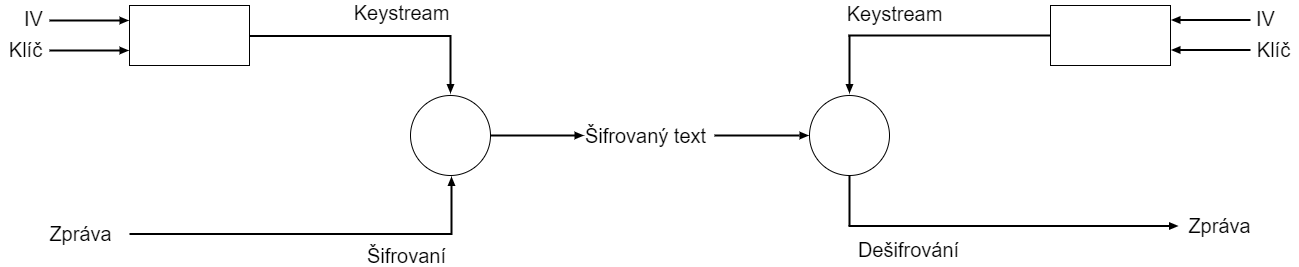
\includegraphics[scale=0.3]{obrazky/synchronousCipher.png}
  \end{center}
  \caption[Synchronní proudová šifra]{Princip šifrovaní a dešifrování synchronních proudových šifer.\cite{EncyclopediaSynchronous}}
  \label{img:synchoronstream}
\end{figure}

U~asynchronních proudových šifer oproti synchronním šifrám je keystream generován šifrovacím algoritmem za pomoci klíče a~předchozích šifrovaných znaků zprávy. Stejně jako u~synchronních šifer by měl být příjemce a~odesílatel synchronizován. Dojde-li však k~desynchronizaci, měla by se šifra sama po několika šifrovaných znacích synchronizovat. Pokud při přenosu nastane chyba, při dešifrovaní několik následujících znaků bude dešifrování provedeno chybně, ale zbytek zprávy bude dešifrován v~pořádku pokud nenastanou další chyby.\cite{HavlicekBakalarka} %TODO veta
\begin{figure}[!h]
  \begin{center}
    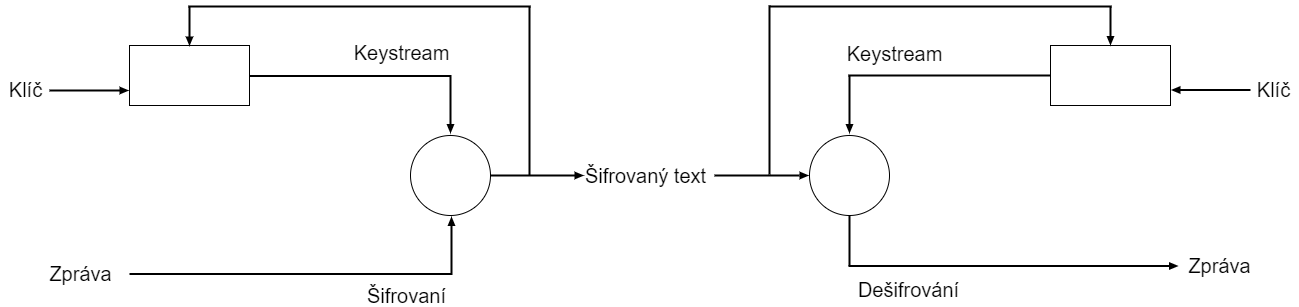
\includegraphics[scale=0.3]{obrazky/asynchronousCipher.png}
  \end{center}
  \caption[Asynchroní proudová šifra]{Princip šifrovaní a dešifrování synchroních proudových šifer.\cite{EncyclopediaAsynchronous}}
  \label{img:asynchronstream}
\end{figure}
% https://doi.org/10.1007/0-387-23483-7_382

\subsection{Blokové šifry \label{subsec:blockFunction}}% možná podsekce symetrických
Blokové šifry na rozdíl od proudových provádí šifrovaní po blocích, kde každý blok je stejně dlouhá n-tice bitů. Moderní blokové šifry jsou založeny na principu kaskádových šifer. Kaskádové šifry fungují na základě řetězení několika šifer. Do následující šifry je vstupním blokem výstupní blok z~předcházející šifry. Poslední výstupní blok je výsledný šifrovaný blok zprávy. V~blokových šifrách se používá princip iterované šifry, která se dělí na Fiestelovu šifru a~substitučně permutační.\cite{Burda9788021446120ISBN}
\begin{figure}[!h]
  \begin{center}
    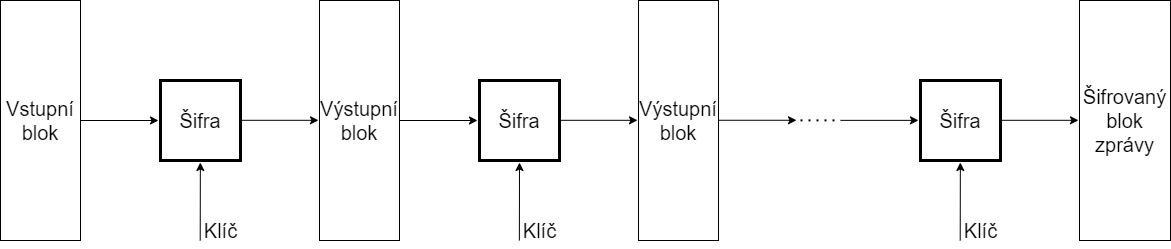
\includegraphics[scale=0.3]{obrazky/cascadeCipher.png}
  \end{center}
  \caption[Kaskádová šifra]{Princip kaskádové šifry.\cite{Burda9788021446120ISBN}}
  \label{img:CascadeCipher}
\end{figure}

Iterované šifry jsou šifry, které využívají princip kaskádových šifer, kdy se využívá zřetězení stejné šifry po několik iterací. Jako šifra pro iteraci se nejčastěji využívá některá z jednoduchých šifer. Z~klíče se odvodí několik iteračních klíčů v~expanzním bloku. Tyto klíče jsou následně použity postupně pro každou iteraci. Jednoduchá šifra společně s~klíčem pomocí vhodných blokových operací jako jsou permutace, substituce a~aritmetické operace, šifrují data do výstupního bloku, který je následně použit jako vstup do další iterace.\cite{Burda9788021446120ISBN}
\begin{figure}[!h]
  \begin{center}
    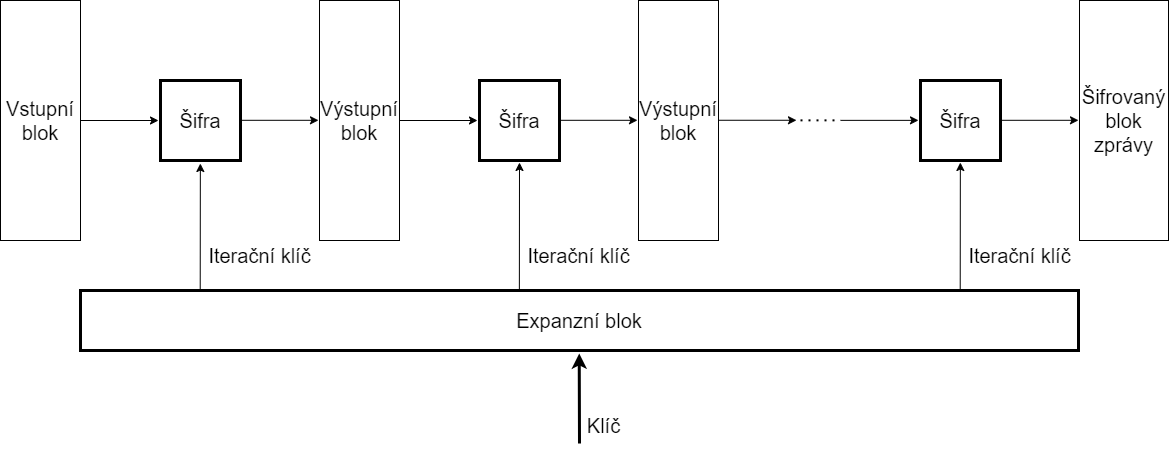
\includegraphics[scale=0.3]{obrazky/IterateCipher.png}
  \end{center}
  \caption[Iterační kaskádová šifra]{Princip šifrovaní iteračních kaskádových šifer.\cite{Burda9788021446120ISBN}}
  \label{img:iterateCipher}
\end{figure}

Prvním typem iterované šifry je Fiestelova šifra. Tento typ šifry funguje na principu rozdělení vstupního bloku na levou a~pravou polovinu. Pravá polovina a~iterační klíč vstupují do konverzní funkce, která má výstup o~délce poloviny vstupního bloku. Výsledkem iterace je blok o~velikosti vstupního bloku, kde novou levou stranou je předcházející pravá strana a~pravou stranou je předcházející levá strana. Jak je patrné, tak šifrována byla pouze levá strana, z~čehož vyplývá, že k~zašifrovaní vstupního bloku jsou potřeba nejméně dvě iterace. Z~tohoto důvodu bývá počet iterací sudý a~dostatečně velký do té míry, aby se zabezpečila difúze šifry.\cite{Burda9788021446120ISBN}
\newpage
\begin{figure}[!h]
  \begin{center}
    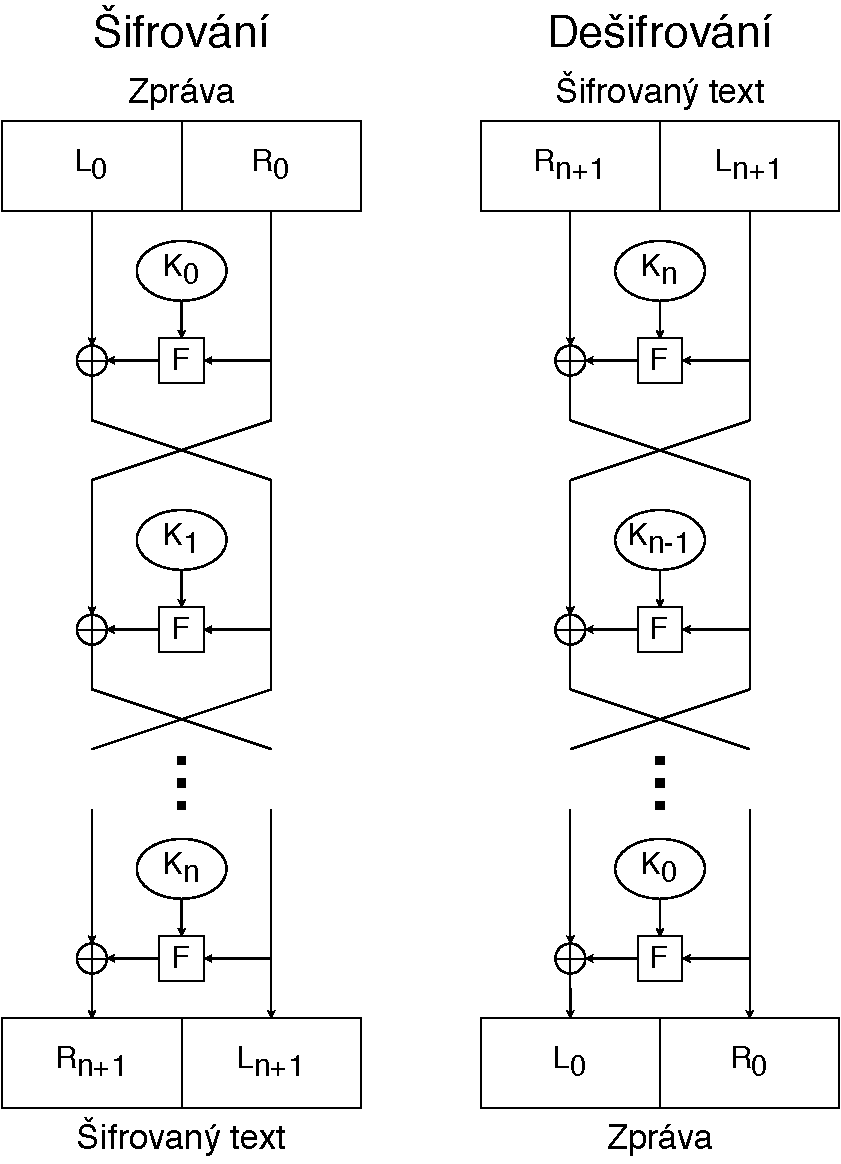
\includegraphics[scale=0.5]{obrazky/feistelCipher.pdf}
  \end{center}
  \caption[Fiestelova šifr]{Princip šifrovaní a dešifrování Fiestelovy šifry.\cite{FeistelCipher}}
  \label{img:FeistelCipher}
\end{figure}
Druhým typem jsou substitučně-permutační síťě zkráceně SPN. Tento typ šifer je založen na substituci a~následné permutaci vstupních bitů. Při substituci se využívá takzvaných S-boxů, které pracují s~částí zprávy, nejčastěji o~velikosti 4 a~8 bitů, kdy se posloupnost těchto bitů nahradí za jinou posloupnost. Permutace se realizuje pomocí takzvaných P-boxů. Permutace se snaží dosáhnout co největší difúze, aby bylo ovlivněno maximální množství S-boxů.%TODO obrazek %file:///C:/Users/Jakub/Desktop/vut_fekt/bajkalarka/zdroje/zaverecna_prace.pdf

Nejčastějšími operacemi používané v substitučně-permutačních síťích jsou:
\begin{itemize}
    \item SubBytes -- nelineární substituce bitů, které operují nezávisle na sobě a~jsou zaměňovány dle předem dané tabulky substituce, která je zároveň klíčem. 
    \item ShiftRow -- v~této operaci se bity posouvají v~řádku matice do stran a~každý řádek se posouvá o~jiný počet míst.
    \item MixColumns -- spočívá v~záměně sloupců, následně je každý sloupec vynásoben polynomem o~stejné hodnotě.
    \item AddRoundKey -- každý byte je zkombinován s~iteračním klíčem, kdy po kombinaci bytů zprávy a~iteračního klíče dostaneme výsledný šifrovaný text. 
\end{itemize}%TODO
%file:///C:/Users/Jakub/Desktop/vut_fekt/bajkalarka/zdroje/final-thesis.pdf
\null
\vfill

\chapter{Lehká kryptografie}
\section{Úvod}
Lehká kryptografie je relativně mladé odvětví, ve kterém se prolíná kryptografie, informatika  a~elektroinženýrství. Zaměřuje se vytváření, adaptaci nebo efektivní implementaci kryptografických primitiv a~protokolů pro zařízení s~omezeným výpočetním výkonem, kterým jsou například mikrokontroléry nebo RFID\footnote{Identifikace na rádiové frekvenci z anglického Radio Frequency Identification} čipy. Z~důvodu omezeného výkonu nelze na tyto zařízení implementovat standartní kryptografické algoritmy.\cite{PoschmannCrypto}

Při návrhu algoritmů lehké kryptografie je nutno udělat kompromis mezi bezpečností, náklady a~výkonem. Tento kompromis lze vidět na \obrazek{img:Compromis}. 
\begin{figure}[!h]
  \begin{center}
    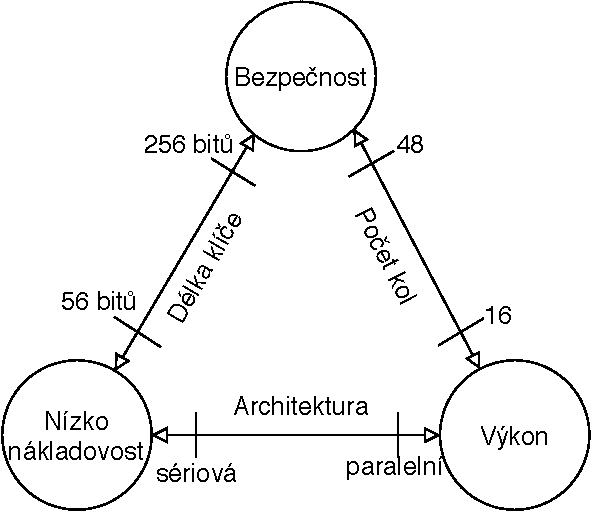
\includegraphics[scale=0.7]{obrazky/designTradeOFF.pdf}
  \end{center}
  \caption[Kompromis při návrhu algoritmu]{Kompromis při návrhu algoritmu.\cite{PoschmannCrypto}}
  \label{img:Compromis}
\end{figure}

Nejčastěji bývají splněny pouze dva ze tří požadavků na návrh algoritmu a to buď bezpečnost a~nízkonákladovost, bezpečnost a~výkon nebo výkon a~nízkonákladovost. Docílení všech tří požadavků tak, aby byli správně optimalizované, bývá velmi náročné. Například vysokého výkonu na hardwaru a~bezpečnosti lze dosáhnout zřetězením architektur, které zakomponovávají několik protiopatření proti útokům postranními kanály. Výsledný návrh bude mít vysoké plošné požadavky, což koreluje s vysokými náklady. Naopak lze navrhnout algoritmus, který je bezpečný a~má malé náklady. Tento algoritmus bude omezen výkonem.\cite{PoschmannCrypto}

Pro zařízení, které využívají lehké kryptografie, byl stanoven požadavek na minimální bezpečnost o~velikosti 80 bitů. Tato délka se zdá být nedostatečná, ale vzhledem k~informaci, která je chráněna, je dostatečná. Při pokusu o~prolomení takového zabezpečení, by útočník musel vynaložit velké úsilí nebo finanční obnos k~prolomení. Zisk z~tohoto pokusu by byl ve většině případů zcela adekvátní.\cite{Klima}

Lehká kryptografie využívá hašovací funkce, proudové a~blokové šifry, které byli speciálně pro tuto potřebu vyvinuty.\cite{Klima}


\section{Hašovací funkce lehké kryptografie}
V lehké kryptografii hašovací funkce fungují na stejném principu jak je uvedeno v~kapitole \fullref{sec:hashFunction}. Jediný rozdíl je v~bitové délce výstupu. V~případě hašovacích funkcí, které se používají na zařízeních u~kterých není omezený výkon, se využívá výstup hašovací funkce o~velikosti 128 bitů a~více. Ve většině případů se přešlo na hašovací funkce typu SHA-256 a SHA-512, které mají délku 256 bitů respektive 512 bitů. Hašovací funkce z~rodiny SHA jsou nejpoužívanější hašovací funkce v kryptografii. 

Lehká kryptografie používá hašovací funkce o~velikosti výstupu 80 bitů a~více. Nejznámějšími hašovacími funkcí je PHOTON, který má více variant délky výstupu.Tyto délky výstupu jsou v rozsahu od 80 bitů do 256 bitů. Další známou hašovací funkcí je SPONGENT, který nabízí varianty výstupu od 88 bitů do 256 bitů.\cite{LightHash}

\section{Proudové šifry lehké kryptografie}
Proudové šifry pro lehkou kryptografii fungují na stejném principu, který je popsán v~kapitole \fullref{subsec:streamFunction}. Proudových šifer pro lehkou kryptografii není navrženo mnoho. Nejpoužívanější šifrou je šifra A5/1, jejíž využití se vyčísluje v~miliardách. Jedním z~důvodů proč jich není vytvořeno mnoho, může být, že stávající proudové šifry jsou několika násobně méně náročné na implementaci. Z~tohoto důvodu lze stávající šifry uzpůsobit její implementaci nebo šifru samotnou tak, aby šifry bylo možné použít na výpočetně omezených zařízeních.\cite{SaldaBP}

Mezi zástupce proudových šifer patří $\mathrm{E_0}$. Tato šifra se často vyskytuje ve sféře mobilních telefonů. Využívá se pro přenos paketů, které udělují důvěrnost při přenosu protokolem Bluetooth. Algoritmus používá klíč, který má délku 128 bitů. Dalším zástupcem je šifra A5/1. Tato šifra se využívá s~sítích GSM a je i~součástí jeho standardu. Využívá 64 bitový klíč a~22 bitový inicializační vektor. Dále byla v~roce 2007 představena šifra Grain, která se využívá hlavně u~zařízení, které mají omezenou paměť a~spotřebu energie. Funguje na principu dvou posuvných registrů a~nelineární funkci, kdy její klíč má délku 80 bitů. Existuje i~verze, která využívá klíč o délce 128 bitů.\cite{SaldaBP} % file:///C:/Users/Jakub/Desktop/vut_fekt/bajkalarka/zdroje/zaverecna_prace.pdf

\section{Blokové šifry lehké kryptografie}
Princip blokových šifer byl detailně probrán v~kapitole \fullref{subsec:blockFunction}. Nejznámější blokovou šifrou, která je založena na principu Fiestelovy šifry, je šifra DES. Z~šifry DES vychází vychází čínská šifra LBlock, která je jednou z~hlavních šifer používaných v~lehké kryptografii a byla navržena pro zařízení s~nedostatkem výpočetního výkonu. Nejznámější blokovou šifrou, která je založena na principu subtitučně-permutační sítě, je šifra AES. Z~této šifry vznikla jedna z~nejznámějších lehkých šifer -- evropská šifra PRESENT. Šifra PRESENT je podobně jako LBlock navržena z~ohledem na zařízení, která mají omezené prostředky výpočetního výkonu.\cite{NekuzaBP}

\subsection{PRESENT}
Šifra PRESENT využívá bloky o~délce 64 bitů a podporuje velikost klíče 80 a~128 bitů. Ve standardu tvůrci navrhují využití 80 bitové varianty. Počet kol opakovaní šifry je 31, v~každém kole je použit klíč určený pro dané kolo, který provádí exkluzivní disjunkci (XOR) na vstupním 64 bitovým blokem. Následně po použití operace XOR se provádí lineární bitová permutace a~nelineární substituce. Nelineární substituce využije jednoho 4 bitového S-boxu, který je použit paralelně 16 krát v~každém kole. Výsledkem bude šifrovaný blok textu.\cite{PRESENT}
%TODO fig.1 from source
\begin{figure}[!h]
  \begin{center}
    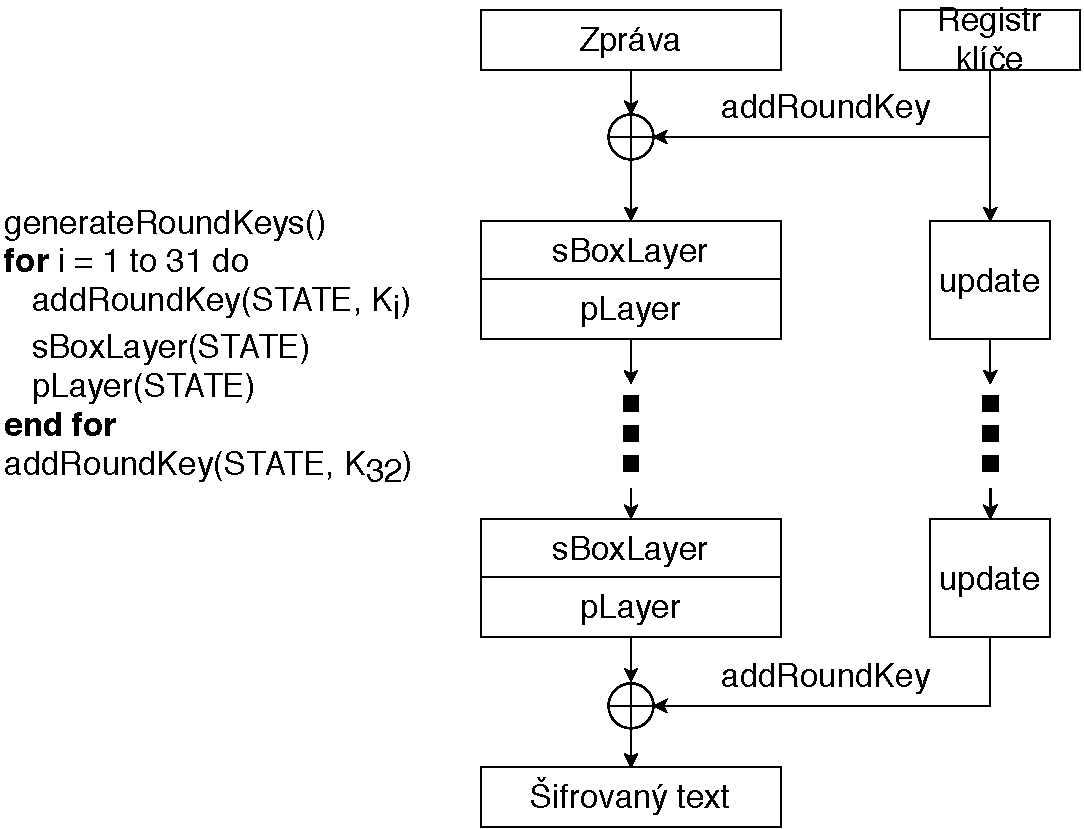
\includegraphics[scale=0.5]{obrazky/present.pdf}
  \end{center}
  \caption[Algoritmcký princip šifry PRESENT]{Algoritmický princip šifry PRESENT.\cite{PRESENT}}
  \label{img:present}
\end{figure}

\noindent \textbf{Substituční vrstva} -- využívá 4 bitové S-boxy, které paralelně nahrazuje. V~\tabulka{tab:SboxTab} je uveden postup nahrazovaní bitů. Na \obrazek{img:present} je tato vrstva označena pod názvem sBoxLayer.\cite{PRESENT}
\begin{table}[!h]
\centering
\begin{tabular}{| >{\centering\arraybackslash}p{8mm} || >{\centering\arraybackslash}p{4mm} | >{\centering\arraybackslash}p{4mm} | >{\centering\arraybackslash}p{4mm} | >{\centering\arraybackslash}p{4mm} | >{\centering\arraybackslash}p{4mm} | >{\centering\arraybackslash}p{4mm} | >{\centering\arraybackslash}p{4mm} | >{\centering\arraybackslash}p{4mm} | >{\centering\arraybackslash}p{4mm} | >{\centering\arraybackslash}p{4mm} | >{\centering\arraybackslash}p{4mm} | >{\centering\arraybackslash}p{4mm} | >{\centering\arraybackslash}p{4mm} | >{\centering\arraybackslash}p{4mm} | >{\centering\arraybackslash}p{4mm} | >{\centering\arraybackslash}p{4mm} |}
\hline
 \textit{x}& 0 & 1 & 2 & 3 & 4 & 5 & 6 & 7 & 8 & 9 & A & B & C & D & E & F \\  \hline
 \textit{S[x]}& C & 5 & 6 & B & 9 & 0 & A & D & 3 & E & F & 8 & 4 & 7 & 1 & 2 \\ \hline
\end{tabular}
\caption[S-box tabulka šifry PRESENT]{\label{tab:SboxTab}Tabulka pro nahrazení S-boxů.\cite{PRESENT}}
\end{table}

\noindent \textbf{Permutační vrstva} -- v~následují \tabulka{tab:PermutationTab} je uveden postup permutace, kdy bit \textit{i}~je předchozí pozice bitu a~\textit{P(i)} uvádí novou pozici bitu. Tato vrstva je označena na \obrazek{img:present} jako pLayer.\cite{PRESENT}

\begin{table}[!h]
\centering
\begin{tabular}{| >{\centering\arraybackslash}p{8mm} || >{\centering\arraybackslash}p{4mm} | >{\centering\arraybackslash}p{4mm} | >{\centering\arraybackslash}p{4mm} | >{\centering\arraybackslash}p{4mm} | >{\centering\arraybackslash}p{4mm} | >{\centering\arraybackslash}p{4mm} | >{\centering\arraybackslash}p{4mm} | >{\centering\arraybackslash}p{4mm} | >{\centering\arraybackslash}p{4mm} | >{\centering\arraybackslash}p{4mm} | >{\centering\arraybackslash}p{4mm} | >{\centering\arraybackslash}p{4mm} | >{\centering\arraybackslash}p{4mm} | >{\centering\arraybackslash}p{4mm} | >{\centering\arraybackslash}p{4mm} | >{\centering\arraybackslash}p{4mm} |}
\hline
 \textit{i}& 0 & 1 & 2 & 3 & 4 & 5 & 6 & 7 & 8 & 9 & 10 & 11 & 12 & 13 & 14 & 15 \\ 
 \textit{P(i)}& 0 & 16 & 32 & 48 & 1 & 17 & 33 & 49 & 2 & 18 & 34 & 50 & 3 & 19 & 35 & 51 \\ \hline\hline
 \textit{i}& 16 & 17 & 18 & 19 & 20 & 21 & 22 & 23 & 24 & 25 & 26 & 27 & 28 & 29 & 30 & 31 \\ 
 \textit{P(i)}& 4 & 20 & 36 & 52 & 5 & 21 & 37 & 53 & 6 & 22 & 38 & 54 & 7 & 23 & 39 & 55 \\ \hline\hline
 \textit{i}& 32 & 33 & 34 & 35 & 36 & 37 & 38 & 39 & 40 & 41 & 42 & 43 & 44 & 45 & 46 & 47 \\ 
 \textit{P(i)}& 8 & 24 & 40 & 56 & 9 & 25 & 41 & 57 & 10 & 26 & 42 & 58 & 11 & 27 & 43 & 59 \\ \hline\hline
 \textit{i}& 48 & 49 & 50 & 51 & 52 & 53 & 54 & 55 & 56 & 57 & 58 & 59 & 60 & 61 & 62 & 63 \\ 
 \textit{P(i)}& 12 & 28 & 44 & 60 & 13 & 29 & 45 & 61 & 14 & 30 & 46 & 62 & 15 & 31 & 47 & 63 \\ \hline
\end{tabular}
\caption[Permutační tabulka šifry PRESENT]{\label{tab:PermutationTab}Permutační tabulka.\cite{PRESENT}}
\end{table}

\noindent \textbf{Key schedule} -- podporuje 80 nebo 128 bitový klíč, v následujícím postupu se zaměříme na 80 bitový klíč. Klíč dodaný uživatelem je uložen v registru klíče \textit{K}, je reprezentován jako posloupnost bitů $k_{79}\,k_{78}\dots k_{0}$. V~kole \textit{i}~se používá klíč, ve kterém je použito prvních 64 bitů z~levé strany uložených v~registru \textit{K}. V~kole \textit{i}~se tedy použije klíč:
\[K_i = k_{63}\,k_{62}\dots k_{0} = k_{79}\,k_{78}\dots k_{16}\]
Po extrakci klíče se registr \textit{K}~upraví:
\begin{align*}
k_{63}\,k_{63}\dots k_{63}\,k_{63} & = k_{18}\,k_{17}\dots k_{20}\,k_{19}\\
k_{79}\,k_{78}\,k_{77}\,k_{76} & = S(k_{79}\,k_{78}\,k_{77}\,k_{76})\\
k_{19}\,k_{18}\,k_{17}\,k_{16}\,k_{15} & = (k_{19}\,k_{18}\,k_{17}\,k_{16}\,k_{15})\oplus \mathsf{round\_counter}
\end{align*}
Registr klíče \textit{K}~je posunut o~61 bitů doleva, první čtyři bity z~levé strany se použijí k~substituci s~S-boxem. V~poslední části se využije operace XOR mezi bity $k_{19}\,k_{18}\,k_{17}\,k_{16}\,k_{15}$ z~registru klíče \textit{K}~a~hodnotou $\mathsf{round\_counter}$, která udává počet kol \textit{i}~které proběhly.\cite{PRESENT}

\newpage
\subsection{LBlock}
Šifra LBlock využívá bloky o~velikosti 64 bitů s~klíčem o~délce 80 bitů. Počet kol opakovaní je 32 kol. V~další části textu budou použity tyto notace\cite{LBlock}:
\begin{table}[!h]
\begin{tabular}{p{15mm} p{8cm}}
\textit{M} & 64 bitová zpráva\\
\textit{C} & 64 bitová šifrovaný text\\
\textit{K} & 80 bitový klíč \\
$K_i$ & 32 bitový klíč pro kolo \textit{i}\\
\textit{F} & funkce pro kolo\\
\textit{S} & S-boxová vrstva \\
\textit{P},\,$P_1$ & Permutační operace pro 32 bitů\\
\shiftleft{8} & bitový posun o 8 bitů vlevo
\end{tabular}
\end{table}

Algoritmus šifrovaní je znázorněn na \obrazek{img:Lblock}. Na začátku šifrovaní se rozdělí zpráva \textit{M} na 2~části $X_1$ a~$X_0$, každá z~částí má velikost 32 bitů. Po posledním kole se výsledné dva bloky $X_{32}$ a~$X_{33}$ spojí do jednoho 64 bitového bloku, který obsahuje šifrovaný text~\textit{C}.\cite{LBlock}
\begin{figure}[!h]
  \begin{center}
    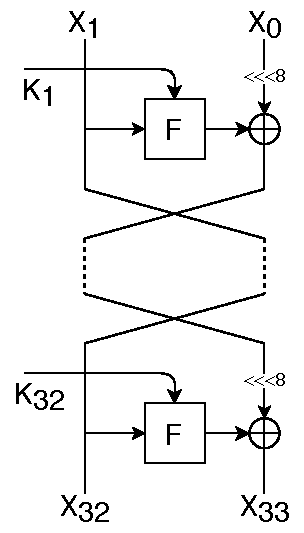
\includegraphics[scale=1]{obrazky/LBlock.pdf}
  \end{center}
  \caption[Algoritmický princip šifry LBlock]{Algoritmický princip šifry LBlock.\cite{LBlock}}
  \label{img:Lblock}
\end{figure}

\noindent Průběh jednoho kola \textit{i} lze vyjádřit jako:
\[X_i = F(X_{i-1}, K_{i-1})\oplus (X_{i-2}<<<8)\]

\noindent \textbf{Funkci kola} \textit{F} lze vyjádřit jako:
\begin{align*}
    \{0,1\}^{32} \times \{0,1\}^{32} & \longrightarrow \{0,1\}^{32}\\
    (X, K_i) & \longrightarrow U = P(S(X \oplus K_i))
\end{align*}

\noindent \textbf{Funkce konfúze} \textit{S} -- obsahuje 8~paralelně poskládaných $4 \times 4$ S-boxů, jejichž obsah je zobrazen v~\tabulka{tab:tableLblock}, kde jsou označeny $s_0\dots s_7$. Každý blok se rozdělí na části o~velikosti 4 bitů. Na každou část je použit S-box. Tímto lze zaručit, že každý bit z~32 bitového bloku bude ovlivněn.\cite{LBlock}
%TODO obrazek roundfucntion
\begin{figure}[!h]
  \begin{center}
    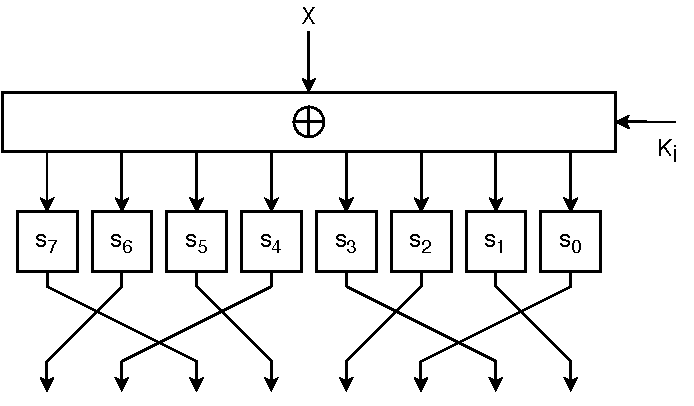
\includegraphics[scale=0.8]{obrazky/RoundLBLOCK.pdf}
  \end{center}
  \caption[Funkce pro kolo šifry LBlock]{Funkce pro kolo šifry LBlock.\cite{LBlock}}
  \label{img:roundLblock}
\end{figure}

\noindent \textbf{Funkce difuze} \textit{P} -- je permutace osmi 4~bitových slov, které jsou výstupem funkce~\textit{S}.

\noindent \textbf{Key schedule} -- 80 bitový klíč \textit{K}~je uložen v~registru klíče $K_r$ jako posloupnost bitů $K = k_{79}\,k_{78}\dots k_{0}$. Klíč pro kolo $K_i$ je vytvořen z~prvních 32 bitů z~levé strany, kde se následovně $K_r$ posune o~29 bitů vlevo. V~další části na prvních 8 bitů z~levé strany jsou použity dva S-boxy $s_8$ a~$s_9$, které lze dohledat v~\tabulka{tab:tableLblock}. V~poslední částí se využije operace XOR mezi bity $k_{50}\,k_{49}\,k_{48}\,k_{47}\,k_{46}$ a~hodnotou \textit{i}, která udává hodnotu aktuálního kola. Výstupem je prvních 32 bitů z~levé strany registru \textit{K}~jako klíč $K_{i+1}$. Postup transformace klíče pro kolo \textit{i}~je zobrazen níže, kde \textit{i}~je pro kola 1~až 31.\cite{LBlock}
\begin{enumerate}[label=(\Alph*)]
    \item $K = k_{79}\,k_{78}\dots k_{49}\,k_{48}$
    \item \textit{K} \shiftleft{29}
    \item $k_{79}\,k_{78}\,k_{77}\,k_{76} = s_9 [k_{79}\,k_{78}\,k_{77}\,k_{76}]$
    \item $k_{79}\,k_{78}\,k_{77}\,k_{76} = s_8 [k_{79}\,k_{78}\,k_{77}\,k_{76}]$
    \item $k_{50}\,k_{49}\,k_{48}\,k_{47}\,k_{46} \oplus i$ 
    \item $K_{i+1} = k_{79}\,k_{78}\dots k_{49}\,k_{48}$
\end{enumerate}

\newpage
\begin{table}[!h]
\centering
\begin{tabular}{| >{\centering\arraybackslash}p{8mm} || >{\centering\arraybackslash}p{4mm} | >{\centering\arraybackslash}p{4mm} | >{\centering\arraybackslash}p{4mm} | >{\centering\arraybackslash}p{4mm} | >{\centering\arraybackslash}p{4mm} | >{\centering\arraybackslash}p{4mm} | >{\centering\arraybackslash}p{4mm} | >{\centering\arraybackslash}p{4mm} | >{\centering\arraybackslash}p{4mm} | >{\centering\arraybackslash}p{4mm} | >{\centering\arraybackslash}p{4mm} | >{\centering\arraybackslash}p{4mm} | >{\centering\arraybackslash}p{4mm} | >{\centering\arraybackslash}p{4mm} | >{\centering\arraybackslash}p{4mm} | >{\centering\arraybackslash}p{4mm} |}
\hline
 $s_0$ & 14 & 9 & 15 & 0 & 13 & 4 & 10 & 11 & 1 & 2 & 8 & 3 & 7 & 6 & 12 & 5 \\ \hline
 $s_1$ & 4 & 11 & 14 & 9 & 15 & 13 & 0 & 10 & 7 & 12 & 5 & 6 & 2 & 8 & 1 & 3 \\ \hline
 $s_2$ & 1 & 14 & 7 & 12 & 15 & 13 & 0 & 6 & 11 & 5 & 9 & 3 & 2 & 4 & 8 & 10 \\ \hline
 $s_3$ & 7 & 6 & 8 & 11 & 0 & 15 & 3 & 14 & 9 & 10 & 12 & 13 & 5 & 2 & 4 & 1 \\ \hline
 $s_4$ & 14 & 5 & 15 & 0 & 7 & 2 & 12 & 13 & 1 & 8 & 4 & 9 & 11 & 10 & 6 & 3 \\ \hline
 $s_5$ & 2 & 13 & 11 & 12 & 15 & 14 & 0 & 9 & 7 & 10 & 6 & 3 & 1 & 8 & 4 & 5 \\ \hline
 $s_6$ & 11 & 9 & 4 & 14 & 0 & 15 & 10 & 13 & 6 & 12 & 5 & 7 & 3 & 8 & 1 & 2 \\ \hline
 $s_7$ & 13 & 10 & 15 & 0 & 14 & 4 & 9 & 11 & 2 & 1 & 8 & 3 & 7 & 5 & 12 & 6 \\ \hline
 $s_8$ & 14 & 9 & 15 & 0 & 13 & 4 & 10 & 11 & 1 & 2 & 8 & 3 & 7 & 6 & 12 & 5 \\ \hline
 $s_9$ & 4 & 11 & 14 & 9 & 15 & 13 & 0 & 10 & 7 & 12 & 5 & 6 & 2 & 8 & 1 & 3 \\ \hline
\end{tabular}
\caption[S-box tabulka šifry Lblock]{\label{tab:tableLblock}S-box tabulka pro šifru LBlock.\cite{LBlock}}
\end{table}
